\chapter{TMTO-Attack}

\label{ch:tmto}

\newpage
\section{Hellman Tables}
\label{sec:hmtheory}
Hellman tradeoff is the first iteration of time memory trade offs, It was first explained in the paper A Cryptanalytic Time - Memory Trade-Off by Martin Hellman.
The idea is similar to a naive table lookup where all possible keys K have been encrypted with the plaintext P. Instead of storing all the key ciphertext pairs which is done in the naive table lookup all pairs are sorted into several chains where the only part stored is the start point and the end point. This way memory is saved but time is increased for the online phase. To find a pair one needs to find the right chain and look up the pair.


\subsection{Precomputation phase} %
Like any other tmto the table itself is generated in the precomputational phase.Each table is fixed for a single plaintext. The plaintext is encrypted with the selected encryption function E, the key is a arbitarily selected from all possible N keys. This results in the ciphertext C which is in turn used as the next key for the next encryption of the plaintext. A reduction function is applied to C which has the purpose to reduce the bit length of C and re-randomize the output.

The Helman tradof has 3 main parameters, m, t and l and they decide the size of the table that will be generated.
m is the amount of rows, t is the columns, and l is the amount of times they are repeated.
Certain requirements are put on these parameters, The size of m*t*t must not be much larger or much smaller than N.
N is the keysize of the cipher we are trying to break. We use a Matrix stopping constant (Hmsc) to hold the difference between N and m*t*t. Hmsc can therefore not be very large nor very close to zero.

add om reduction function

By selecting the parameters the table can be generated. This is done by selecting m random starting points, $ sp^{k}_1,sp^{k}_2,...,sp^{k}_m E N$. Each startingpoint is then used as the start of their chain and with recursion the chain links are computed by $ x^{k}_{i,j}=F_k( x^{k}_{i,j-1})$ for $0<j<=t$. When the endpoint is reached it is stored as a pair with the startpoint ${( sp^{k}_{i}, ep^{k}_{i})}^{m}_{i=1}$.
The Hellman table/matrix is usually visualized like so:
\\
\begin{figure}[th]
  figure from Making better tmto paper
  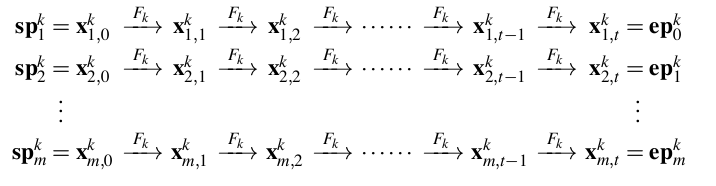
\includegraphics[width=\textwidth]{figures/HellmanMatrix.png}
  \centering
\end{figure}

Here the starting points are sp they are equal to x which is the first element of the chain. It is then encrypted with the current encryption scheme and the reduction function is applied. This is doen t times and $e_t$ is the endpoint.

insert drawing of how Helman chain works
Each row/chain from figure 1 is built the way shown in figure2. E is the encryption K is the key SP start point R reduction function and X is the ciphertext for each chain link. When a table is generated it should contain m touples of (SP,EP) and every chain should contain t+1 keys which results in m x (t+1) keys. This should mean that our tables coverage should be m x t, this is not always the case due to merges.
There are m $x$ t different chain links and it can happen that some of them merge.


\subsubsection{Merges}
Merges happen when in some point of the generation two chains have the same chain link there is a collision and the chains merge. This can be caused by the reduction function, if the reduction function reduces the size of bits of the Ciphertext. If we have ciphertext1 12345678 and ciphertext2 12345679 we have 32 bits here but our encryption only takes 28 bits then this would be a merge if the reduction function just removes the last 4 bit. The chains have now merged and the following intermediate points(chains) will now be the same. This affects coverage, if the merge happens 10 steps into the chain the coverage  will have 10 - t less keys since the two chains will be duplicate.

illustration of merges
\subsubsection{Loops}
Loops occur when a intermediete point(chain link) points back to a previously reached chain link. This also decreases the tables coverage.

figur for chain looping

A loop will loop around in the same chain links untill it reaches t.

\subsubsection{Multiple Tables}
In Hellman as m and t increases it will reach a point where the coverage doesnt increase due to merges and loops. This has been calculated to be somewhere near $N^{\frac{2}{3}}$ for single tables. This is the reason that the upper bounds for M and T are around $N^\frac{1}{3}$

\subsection{Online phase}
Once a table is generated and we have a matching text ciphertext pair (y=F(x)) the online phase can commence.\\
The given ciphertext is used as the key for the encryption and we compute a single chain. This is done the same way as shown in figure 2 each link computed is matched with the computed Hellman table. This is done for all indicies l in the table if a match isnt found the algorithm will report faliure.\\

Whenever a match is found the corresponding SP is returned. The chain is now partially regenerated to obtain $X_{tmp}=x^k_{i,t-j}=F^{t-j}_k(sp^k_i)$. Which should be the key the text was encrypted with:
\begin{equation}
    F^j_k(x_{tmp})=F^j_k(F^(t-j)_k(sp^k_i))=ep^k_i=y^k_j=F^{j-1}_k(y_1)=F^j_k(x)
\end{equation}
\subsubsection{False Alarms}
False alarms happen when in the onlinephase a match is found, but the chain did not contain a valid key. This can happen when a merge has happend earlier when two different chains point to the same end point.
\\
Skal mere paa her
\subsection{Analysis}
This section will address the success probability, cost of resolving alarms, tradeofcurve, memory Usage, precomputational time and online time.


\subsubsection*{Success probability}
The success probability of the table is found by calculalting how many keys that are covered in our table. Increasing the size of the table will increase the probability that the key is in it. The amount of keys that are covered depends on the amount of startpoints and the size of each chain. The success ratio of a single table can be calculated the following way:
Lower bound from hellman paper
$\frac{|HM|}{N}>=\frac{1}{N}\sum^{t}_{j=1}\sum^{m}_{i=1}(1-\frac{it}{N})^{j} $
When the all the tables are prcessed and assuming the reduction functions provide independent results the success probability becomes:
\[1-(1-\frac{|HM|}{N})^l\approx 1- exp(-\frac{l|HM|}{N})\]
Since the count of duplicates is maintained by the matrix stopping rule, the size of the table is :$|HM|\approx mt$.
\subsubsection{Cost of resolving alarms}
The amount of false alarms a table receive is given by $\frac{H_{msc}}{2}$\cite{176} 14, which leads to the cost of resolving them. The cost of resolving alarms are the following:
\begin{equation}
\text{(cost of resolving alarms for all tables)}>=\frac{H_{msc}}{6}lt
\end{equation}
proof found in \cite{176} 18
\begin{equation}
\text{(expected cost of resolving alarms)}=\frac{H_{msc}}{6}t
\end{equation}
proof found in \cite{176} 15
\subsubsection{Tradeofcurve}
The tradeoff curve can be found by applying the matrix stopping rule to M and T.
\begin{equation}
TM^2\approx N^2
\end{equation}
$T=t^2$ and $M=m*t$ When the table is implemented it will take M memory and T time.

Add mere evt om tradeof curves generelt
\subsubsection{Memory Usage}
Storing the table of a tmto such as the Hellman tradeoff takes a lot of space. Therefore it is one of the aspects of the time memory tradeoff to lower the memory cost to a managable size. The hellman tradeoff stores a tuple of a start point and a end point this can be described as $m\cdot mem$ where mem is the bitsize of the  tuple stored. When several tables are used it is multiplied to the previous equation which gives:
\begin{equation}
M=m\cdot n\cdot mem
\end{equation}
where n is amount of tables.
\subsubsection{Precomputational time}
Time spent on generating the tables are also a factor of the tradeoffcurve, the shorter the chains the less time it takes to generate a table. The time spent generating such a table can be computed. There are m different start points and each of them has t chains, this means that we will use $t\cdot m$ encryption's per table. If n tables are generated the formula for the Time the precomputation takes is:
\begin{equation}
  Time=m\cdot t\cdot s
\end{equation}
Time is the amount of encryptions that will take place in the generation of the table. Time is multiplied with the time it takes to do one encryption or devided by the amount of encryptions can be done pr second.

\subsubsection{Online time}
Online time is the time it takes to find a key in the worst case scenario. When searching for a key the worst case scenario is when it takes t applications of F, that is to search through the entire table. If the tradeoff consists of more than one table it is again multiplied by the amount of tables n.
\begin{equation}
  Time=t\cdot n
\end{equation}
The online phase is also multiplied by the time it takes one encryption or divided by the amount of encryptions per second. A major problem in the online phase of the  Hellman tradeoff is the amount of lookups needed. Even if it is possible to compute a million encryptions per second we need the capacity to access our table a million times pr second. And as our table will be stored on the harddrive it will be impossibru.



\section{Distinguished Points}
\label{sec:dptheory}

The distinguished points - tradeof was first described by Rivest in
the book [ref] and was further analysed in \cite{DP}. It is a simple modification of the Hellman tradeoff
where one does not have chains of the same size, since when a
distinguished point is reached the chain does not continue. The way we distinguish any point from a dp by some property (eg. the first 16 bits are zero). This is the DP proporty, with DP-tradeoff the amount of table lookups is lowered dramatically since a lookup only happens when a point that matches the DP property is found.
\subsection{Precomputational phase}
The online phase of the DP-tradeoff is very similar to the Hellman method.
\subsubsection{Parameters}
There are several parameters that decide the size and the coverage of
the DP-tradeoff. M is the amount of rows, t is the chain length  and l is the amount of tables.
To prevent chains from growing uncontrollably $t_{max}$ is used. This is the max size a chain can get before it is aborted and the chain discarded.
Like the Hellman tradeoff the table must satisfy the
given matrix stopping rule $mt^2\approx N$ again the difference between
mt and N should not be too large or to close to zero. Again a
matrixstopping constant is used to hold the difference $mt^2\approx
D_{msc}N$. Reduction functions are selected.... add more. The dp property is given by a bitmask with length $dp_l$.
Once the Parameters have been selected the algorithm can start. $F(SP)=C_1$ is computed and the reduction function is applied which gives the first chain link.$C_1$ is compared to the Dp property, if it is a positive match $C_1$ is an EP this is stored with the SP and the chain length $t_{DP}$. If $C_1$ does not match up with the dp property $F(C_1)=C_2$ is computed and the result compared to the dp property this is done untill an EP is found or the chain length reaches $t_{max}$


\begin{figure}[th]
  DP schema
  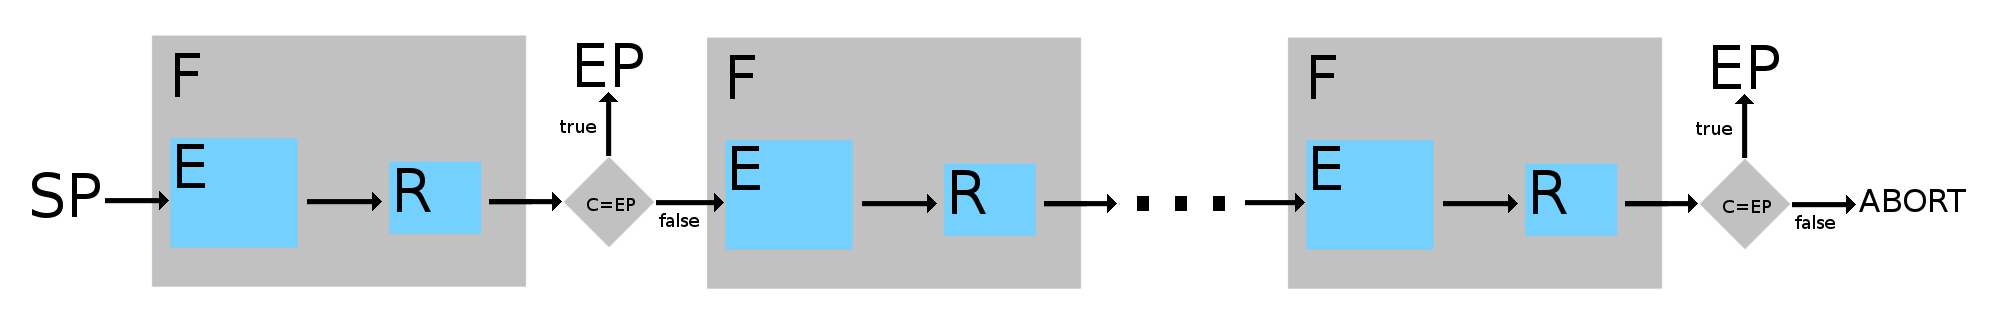
\includegraphics[width=\textwidth]{figures/DPSchema.png}
  \centering
\end{figure}

\subsection{Online phase}
The online phase for the DP-tradeoff is also similar to the Hellman-tradeoff online phase. The major difference is that all EP in the computed table are distinguished points therefore instead of checking all chain links that the given ciphertext gives we only check it when a DP is reached. F is applied to C until a DP is reached or it has been applied $t_{max}-1$ times. If it reaches $t_{max}-1$ the key is not covered in the table but if it is reached we check the table for the distinguished point/EP when found we regenerate the chain from the stored SP, Just like in the Hellman tradeoff. When resolving false alarms we we either have to regenerate the entire chain untill the EP is reached or the $y^k_1$ (WHAT IS THIS). This can be prevented by storing the size of each chain in the table, this wil in turn cause the table to be larger.

\subsection{Analysis}

\subsubsection{DP Property}
The dp property influences the success rate, coverage, precomputation and online time. This means that the property cannot be selected arbitrarily and needs consideration. If the property requirenment is too easily met the length of each chain will decrease, and lead to less coverage since less unique keys will be generated. If it is too hard to meet the chains will become larger but there will be less chains since some will be discarded if a point is not found. Which leads to lower coverage and a longer precomputation time. As stated the length of the dp property matters and influences the coverage and thereby the success rate of a table and can therefore neither be too large or too short. Too long chains are stored to rarely and too short chains do not consist of enough unique chain links.

The dp property also influences the amount of table accesses. When in the online phase a chain is generated until a point where the dp property is met, this means that the probability of a match is related to the property. The probability of finding a match is the following:
\begin{equation}
t(1-e^{-\hat{t}/t})
\end{equation}


\subsubsection{Success Ratio}
The success ratio for the DP tradeoff is given by
\begin{equation}
  D_{ps}=1-e^{-D_{cr}D_{pc}}
\end{equation}
Where $D_{cr}$ is the coverage rate and $D_{pc}$ the pre computational coefficient. Which are found by:
\begin{equation}
  D_{pc}=\frac{mtl}{N}
\end{equation}
\begin{equation}
  D_{cr}=\frac{2}{\sqrt{1+2D_{msc}}+1}
\end{equation}
This is when $\hat{t}$ is sufficiently large, this means that almost all of the chains become distinguished points. For $\hat{t}$ to be sufficiently large it should be larger but the approximation $(1-\frac{1}{t})^{\hat{t}}\approx e^{-\hat{t}/t}$ should still remain valid.
\subsubsection{Memory Usage}
This will only cover for when $\hat{t}$ is sufficiently large.
The memory usage of the distinguished points depends on the generated table. It depends on the amount of start points, m and the bitwise size of the tuple of (SP, EP) mem. The number of tables generated n is multiplied on as well.

\begin{equation}
  M=m\cdot n\cdot mem
\end{equation}

\subsubsection{Precomputation Time}
This will only cover for when $\hat{t}$ is sufficiently large.
Due to the fact that the DP-tradeoff has no fixed chain length each chain takes an individual amount of time when constructed. And it is not allways that the chain is stored, in this case $t_{max}-1$ applications of F has been done for nothing.

\subsubsection{Online Time}
This will only cover for when $\hat{t}$ is sufficiently large.
The online phase for distinguished points is similar to the Hellman Online phase. The length of the initial chain computed is the average of the length of chains in the table L. Which is multiplied to the amount of tables n.
\begin{equation}
  Time=L\cdot n
\end{equation}
The amount of table accesses is where the Distinguished points method really shines since in the worst case it will only do one access per table, and best case only one lookup once a point where the dp property holds has been found.
The probability for p ..




\section{Rainbow Tables}
\label{sec:raintheory}

The last type of dictionary attack we will look into, is the rainbow
attack. The rainbow attack was introduced to improve on the previous
attacks by eliminating the problem of merging chains. In a rainbow
attack the only way a chain will merge, is if a collision happens in
the same row of two pre-computational chains. As the rainbow attack uses different
reduction functions for each row of the chain, collisions happening
any other place will simply continue with different reduction
functions.

Because of this property rainbow tables will also be loop free. This
will save a lot of work compared to the two other discussed attacks.

For the rainbow attack, we will consider tables with $m$ entries build
from $t$-long pre-computational chains. The parameters $m$ and $t$
will be set such that an attack on a cryptographic
function with key size \textbf{N}, will satisfy the matrix
stopping rule $m \cdot t \approx \textbf{N}$. A matrix stopping $R_{msc}$
constant is introduced which will fulfill $m\cdot t = R_{msc} \cdot
\textbf{N}$. Another big difference between the rainbow attack and the
other discussed attacks is the small number of tables $l$, often only
one large table. As for our calculations we will mostly be looking at
rainbow attacks with only one table if nothing else is stated.

\subsection{Pre-computation Phase}

A Rainbow table is build with $m$ entries of end points, where each endpoint
$ep$ in the table is computed by a $t$ long pre-computational chain.

Each endpoint of a row is computed from a chosen/randomly chosen
start point $sp$. From the start point $sp$ the pre-computational chain,
which generates our endpoint, is computed.

For Rainbow tables, the main difference compared to the other
discussed TMTO-attacks is the reduction function. Rainbow attacks
uses $t$ different reduction functions $R_1,R_2..R_t$ to compute a pre-computation
chain of length $t$.

See \ref{fig:rainbowchain} for the structure of an $i$-th
pre-computational chain of a rainbow table.

\begin{figure}[H]
  \centering
  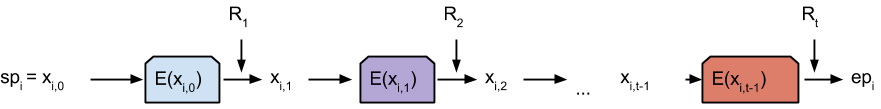
\includegraphics[scale=0.4]{figures/rainbowchain.png}
  \caption{Rainbow Chain - shows weirdly in report Fix?}
  \label{fig:rainbowchain}
\end{figure}

A full rainbow table consists of $m$ iterations of the rainbow chains,
with $m$ different starting points.

If no other means of storage optimization is done, each chains
starting point and ending point is stored in the rainbow table.

The pre-computation phase of a rainbow attack requires 
$R_{msc} \cdot \textbf{N} \cdot l$ calls to the cryptographic function the attack targets. 

\subsection{Online phase}
\label{sec:onlinerb}

The online phase of the rainbow attack differs from the other
discussed TMTO attacks, as $t$ reduction functions are used to
generate the table. To look up a key in the rainbow table one has to
compute the online chain for an input $c$. The online first element of
the online chain is computed by $R_t(c)$ and looked for in the
table. If no match is found the next element $R_t(f(R_{t-1}(c)))$ is
computed and checked for a match then $R_t(f(R_{t-1}(f(R_{t-2}(c)))))$
and so on. If an element is found the reconstruction of the chain with
the matching end point is then done from the corresponding start
point. If the key is not found in the recounstructed chain we will see
this as a false alarm. If the key is found the attack was a
success. This type of table lookup will leave us with at most
$\frac{t(t - 1)}{2}$ calculations of the cryptographic function and
$t$ lookups in the the table.

\subsection{Analysis}

Same as the other?



%%% Local Variables:
%%% mode: latex
%%% TeX-master: "Thesis"
%%% End:
